\chapter{Related work}
In this chapter we survey the studies which focus on problem of irradiance estimation using sky images. The usage of ground-based cameras for studying effect of clouds on irradiation has a long history, as early as 1977 when Borkowski et al.\cite{Borkowski1977} developed the first whole-sky camera system for investigating effects of clouds on middle ultraviolet global radiation. In this study, the degree of solar obstruction and cloud coverage were determined visually from the images. Later in 1998, Jeff Sabburg and Joe wong\cite{Sabburg1998} developed and evalued the first automated, ground-based, sun-centered sky camera system for cloud assessment. However, since the purpose of study was the clouds effect on UVB\footnote{Ultraviolet B} radiation they only considered a small area around the sun for cloud and sun obstruction detection which is of paramount importance for this rays. They use a threshold-based approach on gray scale pixel intensities for cloud detection. They also use solar radiation measurements in a image processing algorithm to reduce reflections from the sun on the camera system being mistaken for cloud in the images.

\section{Estimate irradiance from zone types in sky images}
One of the recent researches done in this area is held as a collaboration between Universitatea Transilvania din Braşov in Romania and Cyprus University of Technology\cite{romania_paper}\cite{romania_report}.This work uses sets of two consecutive images taken by wide-view angle GoPro Hero2 camera(one with normal exposure and the other one under-exposed) and extracts their RGB\footnote{(Red, Green, Blue)}, HSV\footnote{(Hue, Saturation, Value)} components. Then by learning several intensity ranges, they segment four zone type in each image: sun, blue sky, thin clouds and thick clouds. One sample of segmentation is shown in figure\ref{fig:capatitati}.

\begin{figure}[h]
\caption{Three different zones identified in images (sun, cloud, sky)}
\label{fig:capatitati}
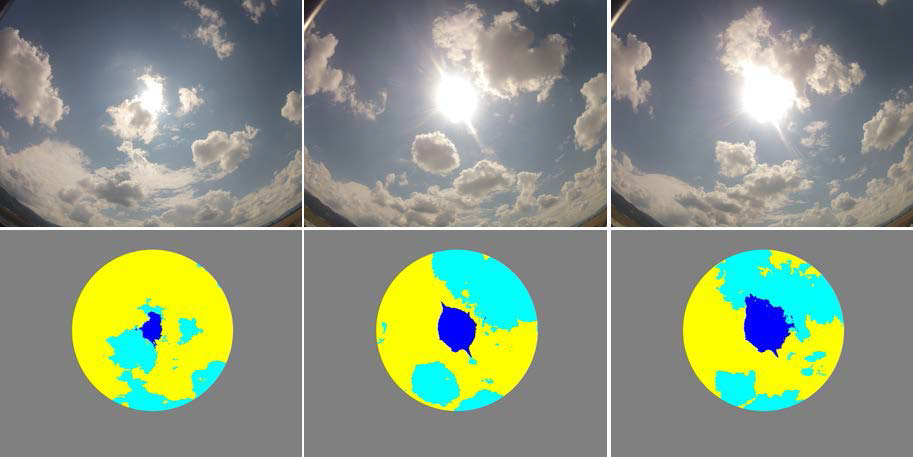
\includegraphics[scale=.5]{capatitati}
\centering
\end{figure} 

 The irradiance (direct, diffuse, global) is recorded using the equipment Kipp \& Zonen, Solys2 at the same time of image capturing. Finally, a regressor used to estimate direct irradiation (DNI) based on a feature vector consisting the number of pixels of different zone types in the images. The correlation in the result is shown in figure\ref{fig:w1_predict}.

\begin{figure}[h]
\caption{Correlation between estimated DNI and recorded DNI.}
\label{fig:w1_predict}
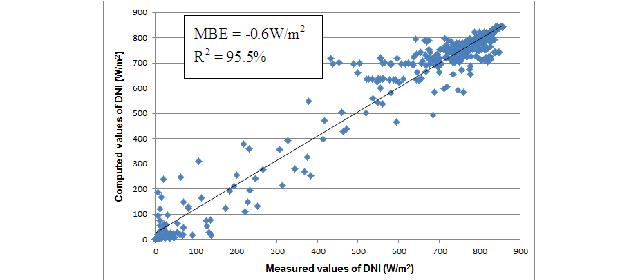
\includegraphics[scale=.7]{w1_predict}
\centering
\end{figure} 

\section{Using clear sky irradiance model and binary cloud mask}
The work done by T. Schmidt et al.\cite{tSchmidt_full} at University of Oldenburg in Germany is a very recent and relevant work on irradiance forecast using sky imager pictures. The experimental setup consists of a wide-view camera, one ceilometer (cloud base height sensor) located next to the camera, and a grid of 99 pyranometer distributed uniformly over 10km by 12km in the area close to camera. The aim is to forecast irradiance of every pyranometer up to 30 minutes. The training data is recorded from the pyranometers and the camera for two months every 10 seconds during daytime.
In order to determine clouds projection on the ground, they apply a series of image processing algorithms. 
\subsection{Cloud detection}
Firstly, they use Red-to-Blue Ratio (RBR) threshold for cloud detection which was first developed by Scripps Institution of Oceanography \cite{RBR89, RBR98} and is been used in many sky-imager-based forecast applications such as \cite{cloud_detection_using_RBR}.  The RBR values close to 1 are usually cloud, and values very less than 1 are blue sky, since the blue channel which is in denominator dominates the red channel. However, since the RBR is not homogeneously distributed over the whole field of view, using a fixed global threshold for cloud detection brings a lot of misclassification for the areas close to the sun and also dark thick clouds or very transparent clouds. Therefore, they correct the RBR values based on clear-sky RBR values for each pixel. A Clear Sky Library (CSL) is created from images of one clear day. Then, the closest distance of current position and sun positions of CSL images is used to choose the reference RBR image map. This RBR map is used in correction formula \ref{eq:RBR_correction} to decrease RBR threshold in circumsolar area to counter effect of sun saturation there. The correction also decreases RBR threshold for dark areas and increases it for bright pixels of image in order to detect thick and thin clouds.
\begin{equation}
\label{eq:RBR_correction}
R_{mod,i,j} =  R_{orig,i,j} - R_{CSL,i,j} \times (a \times S - b \times (I_{i,j} - 200))
\end{equation}
Where $0<S<1$ is the average pixel intensity in circumsolar area. For more detailed discussion on results, they also apply a image-based cloud type classification using several visual cloud characteristics , and classify them into 7 different cloud types.

\subsection{Image un-distorion}
\label{sec:image_undistortion_schmidt}
Since the raw image is from a fisheye lens, they apply a transformation to project it into geometric coordinates for convenience in other calculations. For that, intrinsic parameters of camera are determined using Scaramuzza Matlab toolbox \cite{fisheye_undistort} which solves a fifth-degree polynomial function of point-mapping between fisheye image and plain image. The extrinsic parameters are calculated as the best rotation which matches position of sun re-projection (derived mathematically) and sun position in the image. They calculate sun zenith and azimuth by using solar geometry2 algorithm\cite{sun_pos1}.

\subsection{Shadow mapping}
In this step, shadow of cloud pixels are projected on the ground. For this, besides incidence and azimuth angle of every cloud pixel (which is derived using camera calibration function), cloud base height is needed. The cloud base height is estimated using a ceilometer for every point in time. However, to smooth th data, median of last 30 measurements is used. Even though the ceilometer supports multi-layer clouds as well, in this work they only use the lower-level cloud height. The distance of every cloud pixel to the camera is derived using $d_{i,j} = h \times tan(\theta_{i,j})$. Given the distance $d_{i,j}$, incidence angle $\theta{i,j}$, pixel's azimuth angle $\phi_{i,j})$ and current sun position angles, horizontal distance of the cloud's show on the ground from the camera is calculated using Eq. \ref{eq:shadow_map}.
\begin{equation}
\label{eq:shadow_map}
\begin{split}
dx_{i,j} = h \times tan(\theta_{i,j}) \times sin(\phi_{i,j}) + h \times  tan(\theta_{sun}) \times sin(\phi_{sun}) \\
dy_{i,j} = h \times tan(\theta_{i,j}) \times cos(\phi_{i,j}) + h \times  tan(\theta_{sun}) \times cos(\phi_{sun})
\end{split}
\end{equation}
The shadow pixel points are mapped to a grid of 20km to 20km with resolution of 20m, and coordinates are interpolated if the shadow map resolution is lower than grid resolution, otherwise the central pixel of the dense shadow area is used for that grid point. Finlay, a Gaussian filter is applied to smooth the cloud edges for more realistic result.

\subsection{Irradiance retrieval}
Upon determining the shadowed and sunny grid points on the ground area of experiment, they use the histogram of clear-sky index ($k^{*}$) to estimate the GHI irradiance. The clear sky index is defined as ratio of measured global horizontal irradiance $GHI_{meas}$ and a clear sky reference value $GHI_{clear}$ (Eq. \ref{eq:clear_sky_index}).
\begin{equation}
\label{eq:clear_sky_index}
k^{*} =  \frac{GHI_{meas}}{GHI_{clear}}
\end{equation}
Clear sky irradiance is obtained from the mode of Dumortier \cite{clear_sky_model} and turbidity values of Bourges \cite{turbidity} which is validated according to Ineichen's work \cite{Ineichen}.
For adapting to smooth changes of irradiance caused by factors other than clouds, this histogram is generated with measurements of last 30 minutes. As it is shown in figure \ref{fig:hist_k_index} this histogram usually has two peaks which correspond to sunny and shadow states on the specified point of ground. Now, for every point on the ground, based on its state (shadow, no-shadow), the corresponding $k^{*}$ is used from the peaks of the histogram to estimate GHI following Eq. \ref{eq:calc_GHI}. In case two distinct peaks could not be detected in histogram due to homogeneous irradiance condition, default values of 0.4 and 1, have been assigned for shadow and no-shadow states.
\begin{equation}
\label{eq:calc_GHI}
GHI = k^{*}_{hist} \times GHI_{clear}
\end{equation}

\subsection{Irradiance forecast}
For forecasting the cloud map, they use optical flow algorithm (Lucas-Kanade) on cloud edges and corners (Shi-Tomasi method) in the past 2 minutes to extract clouds' motion vector. Then, by applying that motion vector to current cloud state, cloud map at different time horizons is estimated, and ray tracing from sun position at that times through cloud maps gives the shadow map on the ground. After determining shadow or no-shadow states for points on the ground, forecast GHI is estimated using Eq. \ref{eq:calc_GHI} . They compare results of using GHI histogram from the nearest pyranometer station versus using only the pyranometer close to the camera as a representation for the whole area. These comparison is separately done for different cloud types, and the results shows for cumulus clouds using one pyranometer close to camera is enough to forecast irradiance for up to 2km radius. However, the forecast skill is highly varies depending on cloud types and overall does not do better than persistent model which uses median of past several minutes' irradiance.


\section{Retrieval of direct and diffuse irradiance from sky images}
In another recent work, T. Schmidt et al.\cite{tSchmidt15} aims to estimate components of irradiance (direct, diffuse) instead of just GHI from the sky images using machine learning on image features. They hope this kind of irradiance detail helps in estimating GHI in cloudy and partial sunny states more accurately. The Experimental setup includes a fish-eye camera  with sample rate of 10 sec and a pyranometers package next to it that records direct, diffuse and global irradiance every second. 
\subsection{Image features}
As image features they calculate several local and global features including: 
\begin{itemize}
\item Texture properties of the Grey Level Co-occurrence Matrix (GLCM)
\item Color statistics (RGB space)
\item Inter-color relations ( e.g. Red-Blue-Ratio)
\item Statistics of saturated pixels in circumsolar area in RGB and HSV color space
\item Derived features like cloud coverage
\item Solar elevation angle
\end{itemize}
For prediction, two k-nearest-neighbor (kNN) models are trained that estimate the clear sky index of diffuse horizontal ($k^{*}_{DHI}$) and direct normal ($k^{*}_{DNI}$) components which are defined as ratio of each component to their clear-sky values obtained from Ineichen's algorithm\cite{Ineichen}.
Since the initial feature list contained 37 features, for reducing computation time and avoiding over-fitting they apply a feature selection using decision tree feature ranking algorithm to choose the optimal feature set among them. 
\subsection{irradiance estimation}
The result of KNN predication for DHI and DNI clear-sky indexes compared to measured values shows a correlation around .085 in Figure \ref{fig:knn_result_Schmidt}. In forecast applications, GHI can be derived from predicted irradiance components using \ref{eq:irr_components}. However, predictability of some of the used image features such as color statistics in this method is not robust enough. This leads to some errors in irradiation forecast.

\begin{figure}[h]
\caption{Comparing estimated  $k^{*}_{DHI}$ and $k^{*}_{DNI}$ to measured values.  source:\cite{tSchmidt15}}
\label{fig:knn_result_Schmidt}
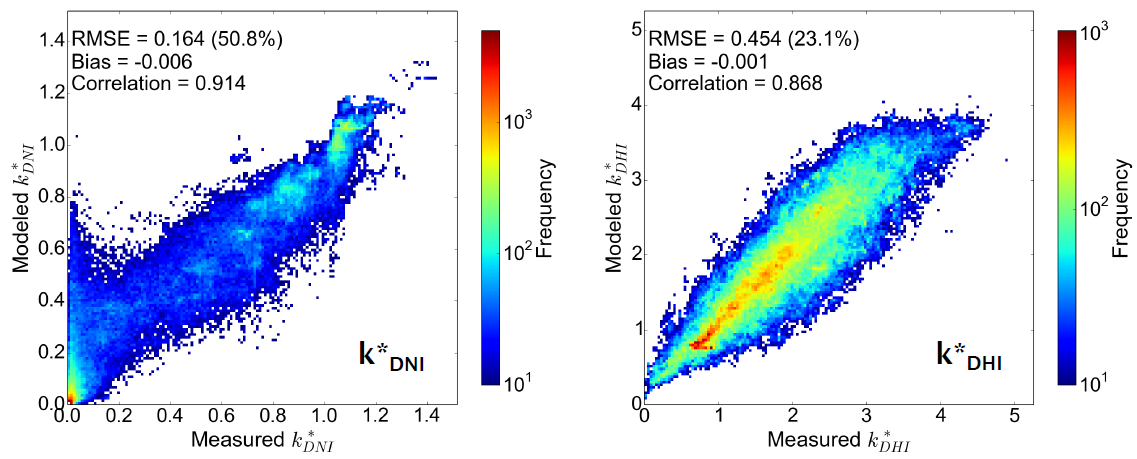
\includegraphics[scale=.44]{schmidt_knn_result}
%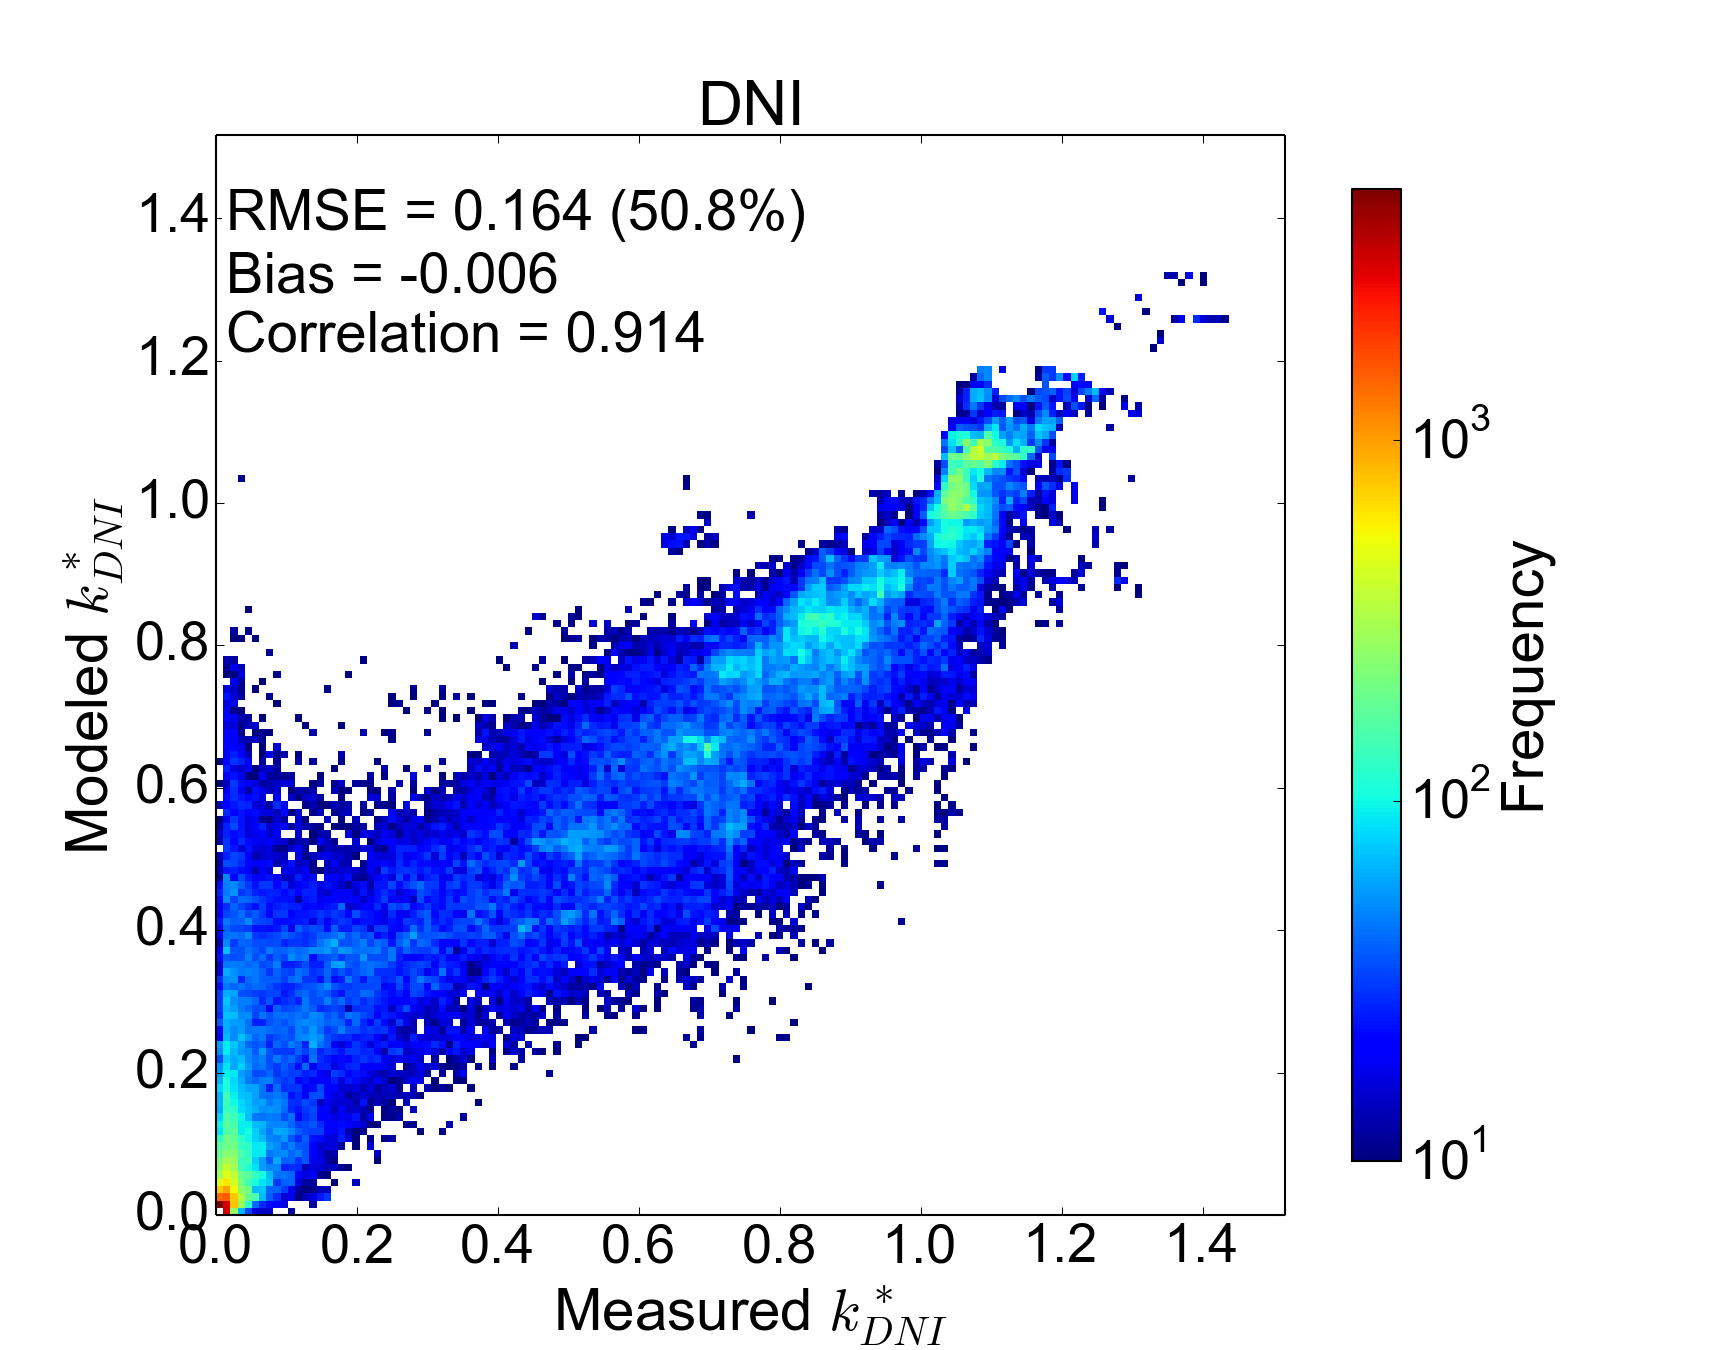
\includegraphics[scale=.2]{schmidt_knn_DNI}
%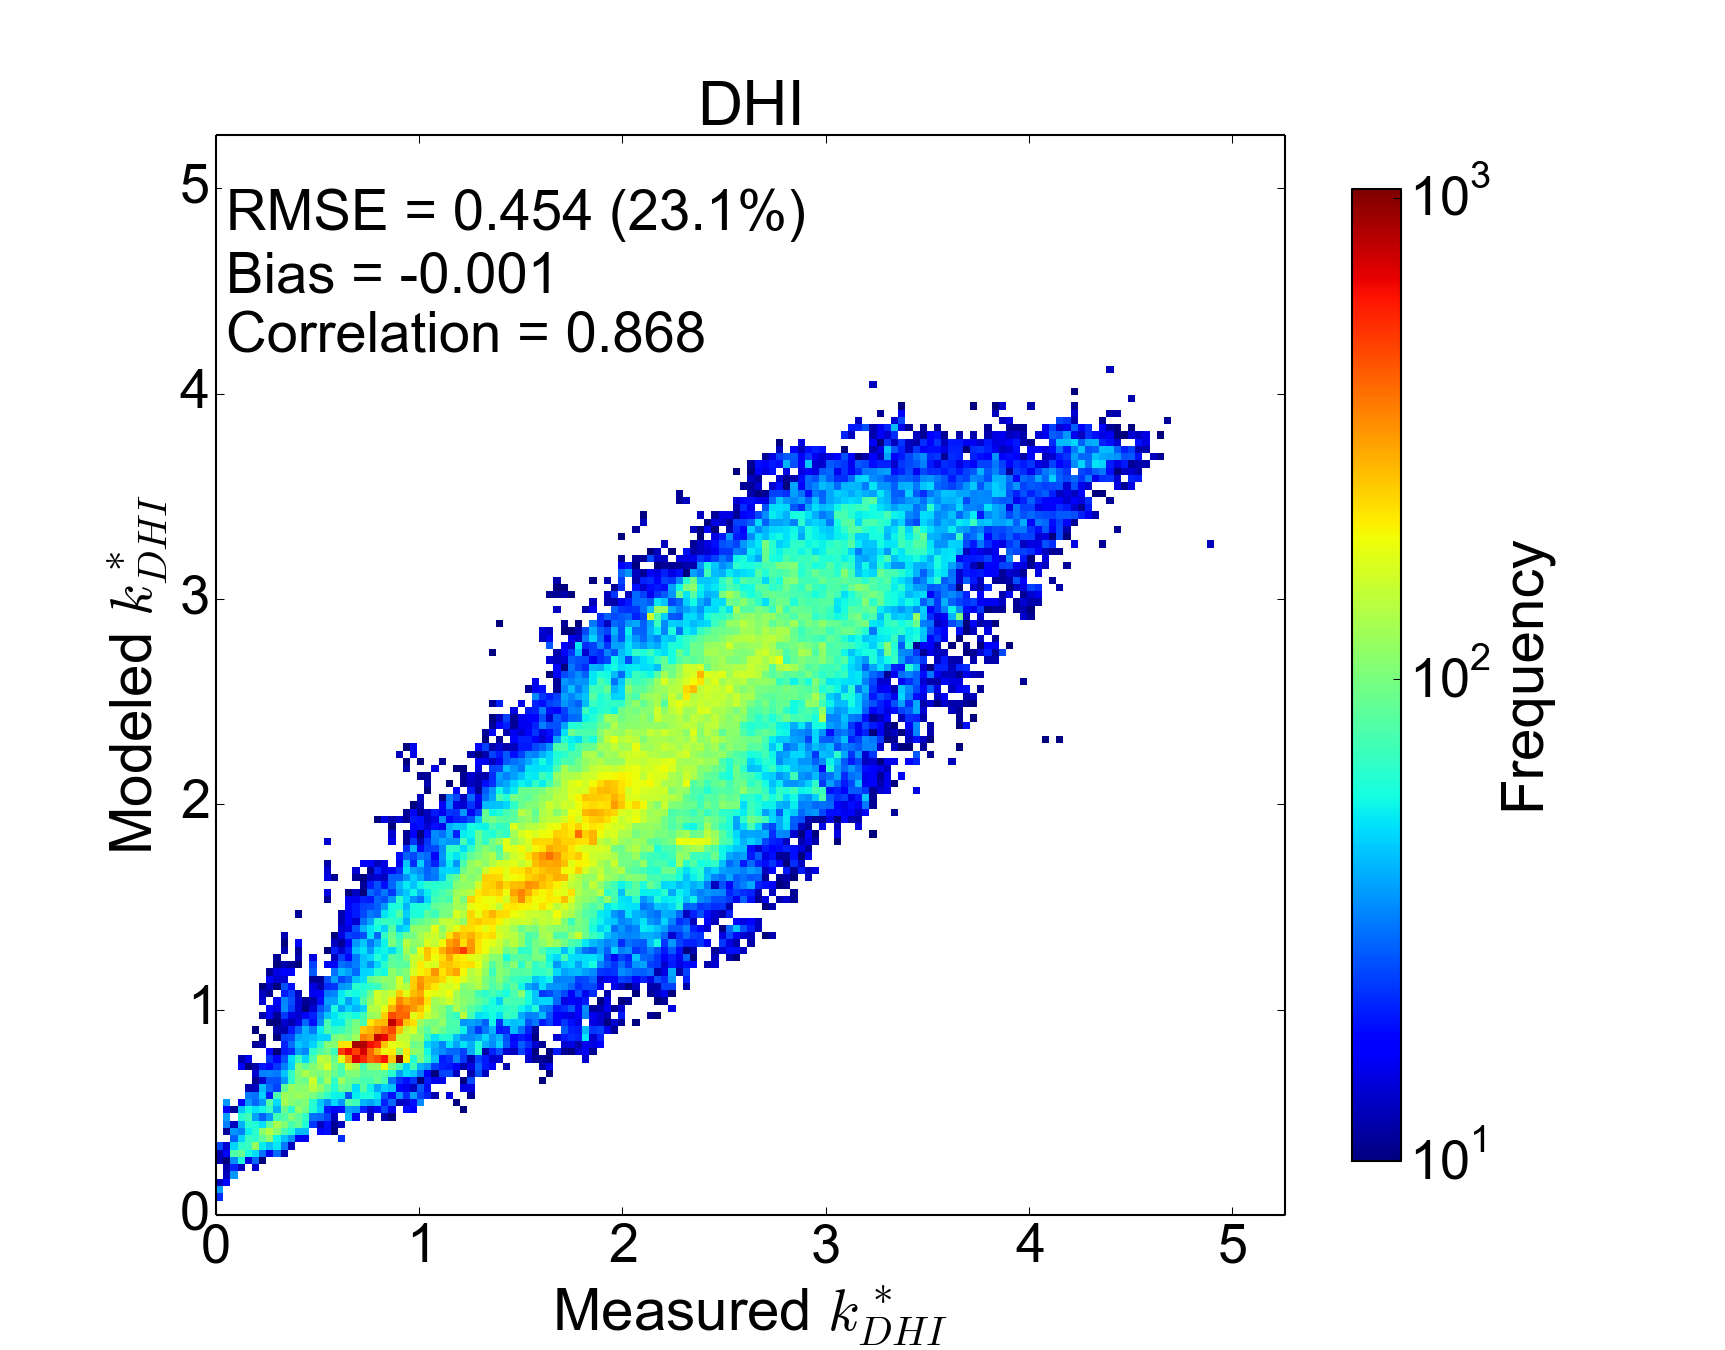
\includegraphics[scale=.2]{schmidt_knn_DHI}
\centering
\end{figure} 
 